%!TEX root = Tesi__Simone_Mariotti.tex
\chapter{Componenti hardware}
\fancyhead[R]{\bfseries Componenti hardware} 	 	
\fancyfoot[C]{\thepage } 
\section{UDOO Quad}
UDOO è un progetto tutto italiano di una piattaforma hardware destinata alla 
generazione dei ``makers'', i cosiddetti \emph{artigiani digitali} del 21$^\circ$ secolo,
cioè persone che inventano e producono apparecchi di ogni genere e condividono i risultati 
pubblicamente sotto licenza open-source così che possano essere la base di un 
progetto di un altro maker. La 
scheda ha visto la luce dopo una sorprendente campagna di crowdfunding
\footnote{Dall'inglese crowd, folla e funding, finanziamento. In italiano 
finanziamento collettivo. La piattaforma utilizzata è Kickstarter.} che ha raggiunto la quota richiesta dagli sviluppatori 
per iniziare la produzione in solo due giorni. 
Per permettere l'utilizzo di librerie e applicazioni computazionalmente pesanti 
come openCV, PureData e altre UDOO è dotata di un processore ARM Freescale i.MX6 
Cortex-A9 Quad core 1GHz che supporta sia Android che Linux. Il tutto è 
completato da una GPU Vivante, 1GB di RAM DDR3, connettore SATA, ingresso microfono, 
uscita audio, Ethernet, HDMI, USB, connettore per display LVDS 
con touch screen, connettore CSI per camera esterna e connettività bluetooth e 
Wi-Fi. La board supporta i sistemi operativi Linux ed Android nelle rispettive 
versioni compilati per i processori ARM. Il sistema operativo risiede su una memoria 
microSD e il caricamento viene eseguito grazie ad un lettore di schede microSD integrato. 
Quello che però ha fatto di questa scheda la nostra scelta per questo 
progetto di tesi, è la presenza all'interno di un Arduino Due completamente integrato.
È presente una CPU Atmel SAM3X8E ARM Cortex-M3 \footnote{La stessa di cui 
dispone l'Arduino Due.} e 76 GPIO\footnote{General Purpose Input/Output.}, di 
cui 62 digitali e 14 digitali/analogici, disposti per essere perfettamente 
compatibili con la piedinatura dell'Arduino Due e dell'Arduino Uno Rev.3.

\begin{figure}[!htb] \center
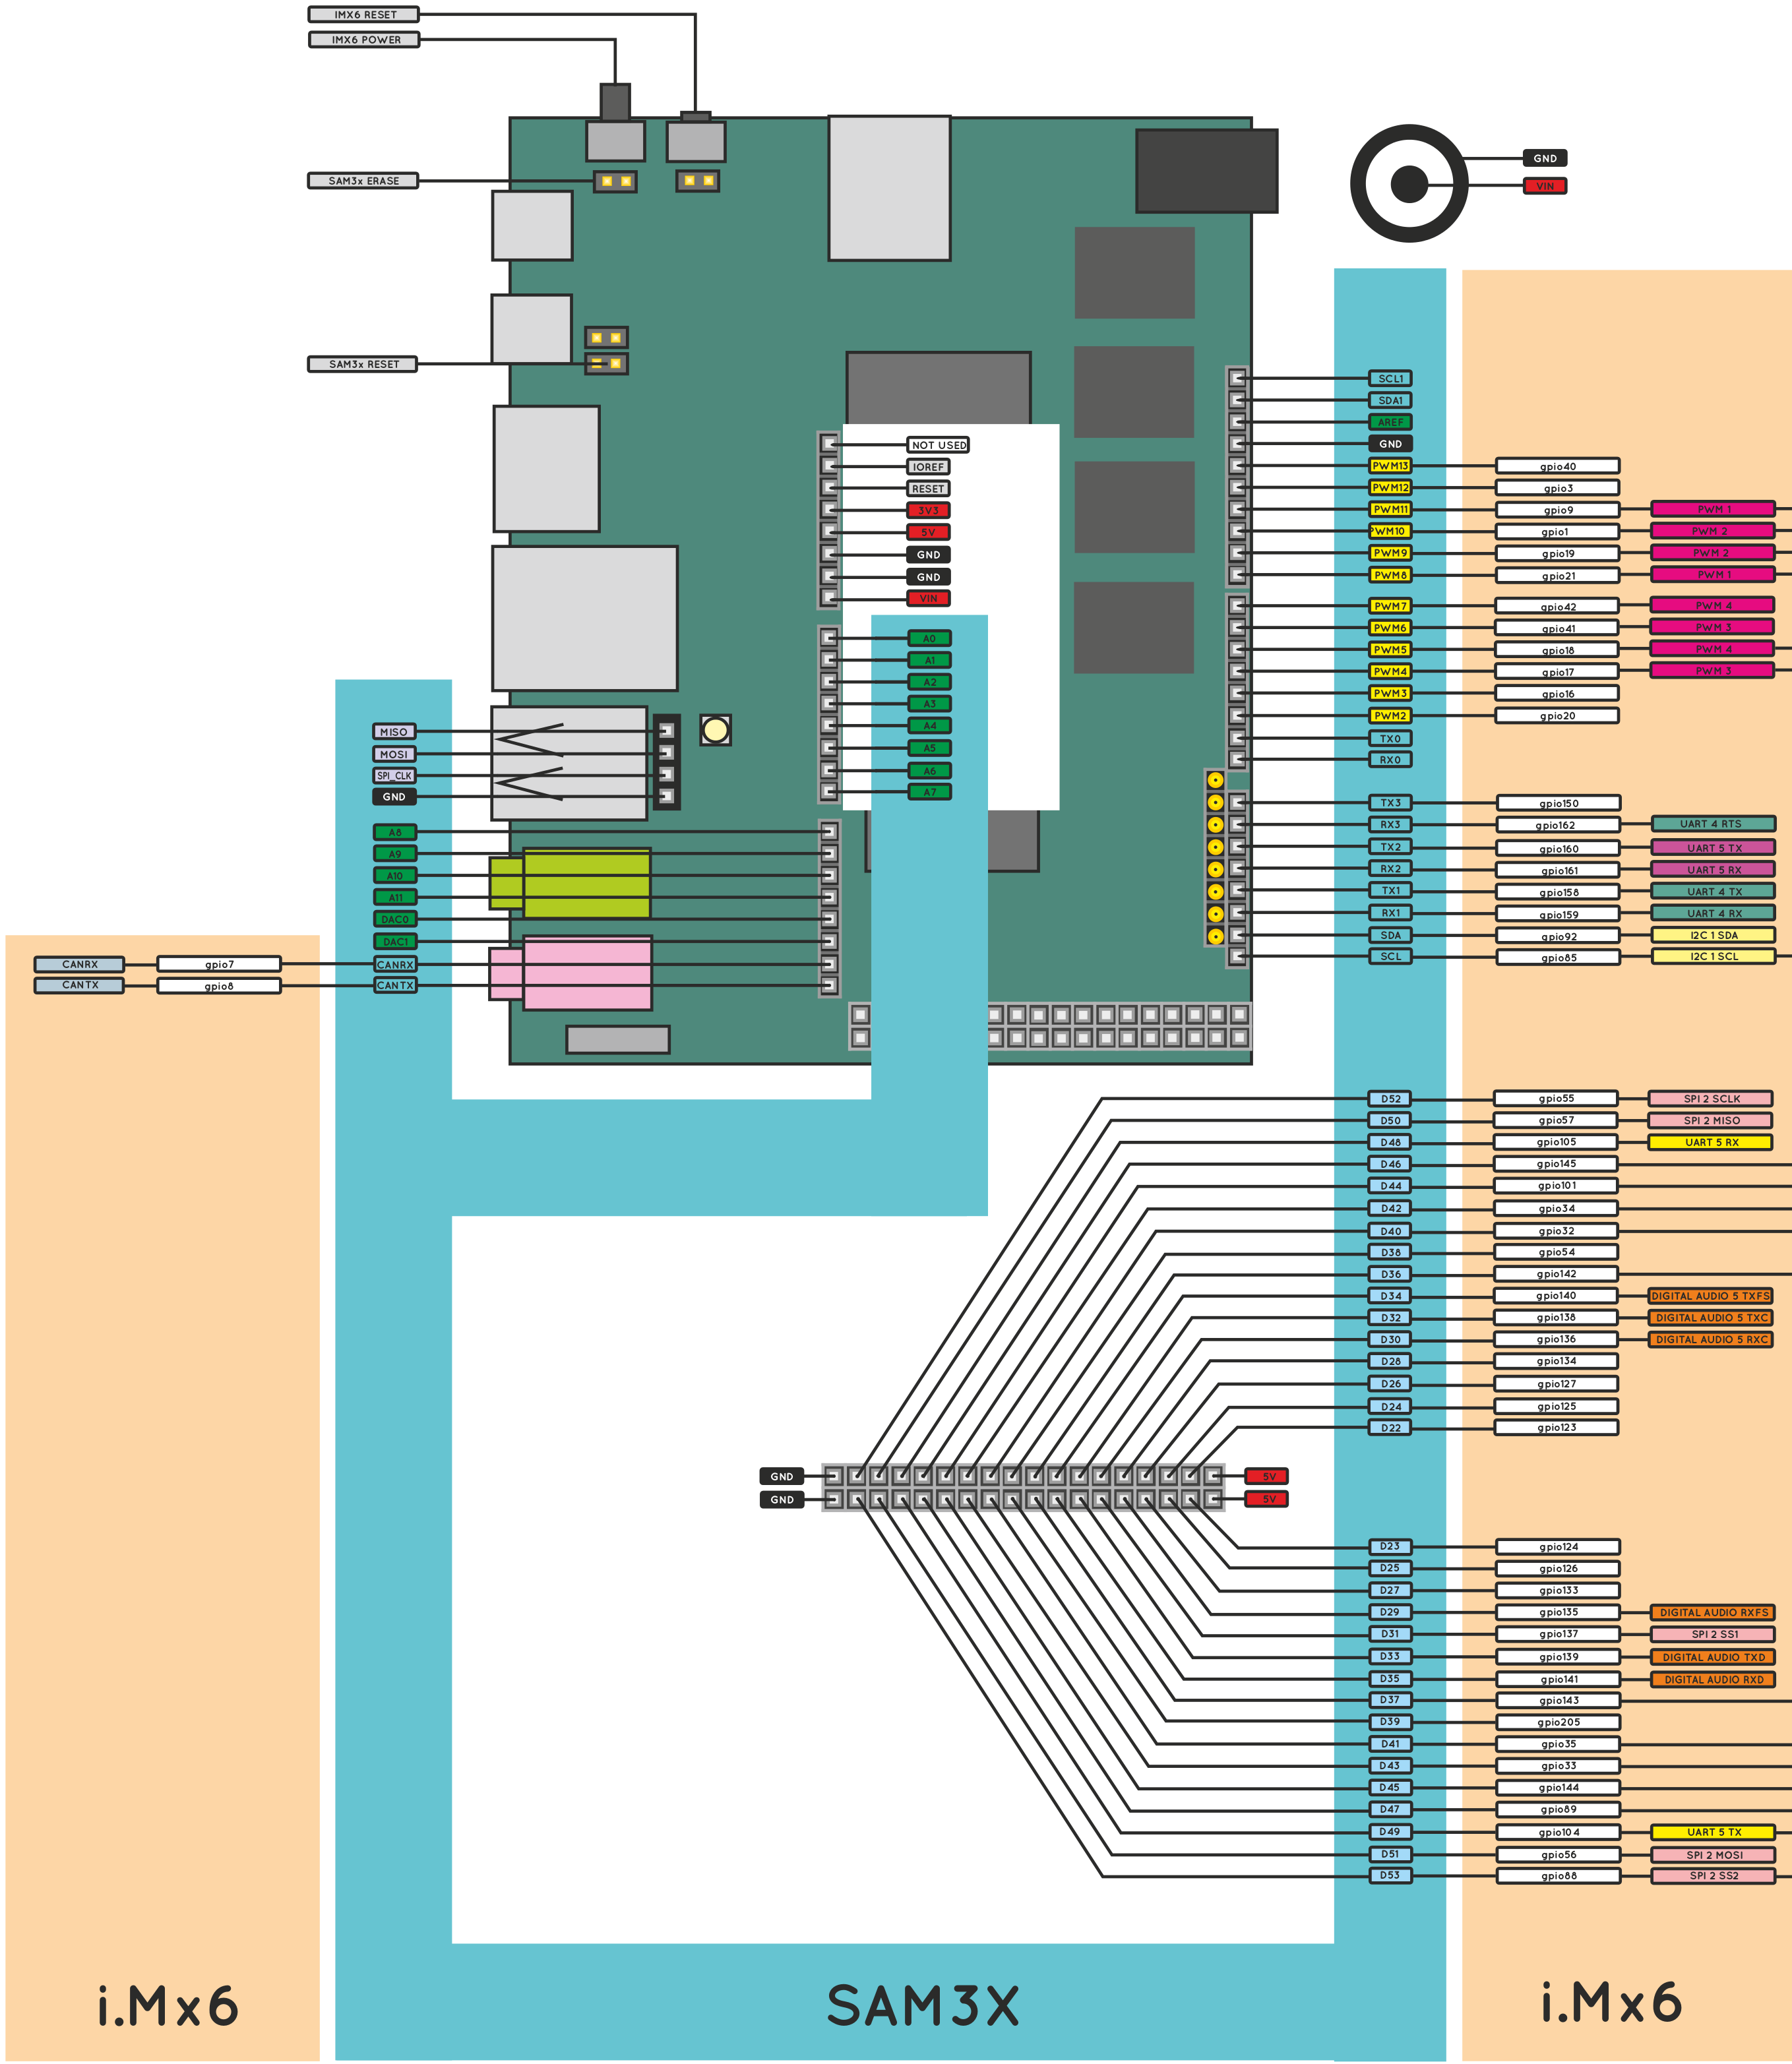
\includegraphics[width=\textwidth]{immagini/udoo_pinout.png}
\caption{Schema piedinatura UDOO} 
\end{figure}

La presenza di un Arduino Due all'interno della board rende UDOO una scheda di 
prototipazione a tutti gli effetti, aprendo nuovi scenari e 
possibilità grazie alla versatilità e semplicità di Arduino, la potenza di 
calcolo del Freescale i.MX6 e le numerose periferiche disponibili per Linux o 
Android.\\
È possibile accedere alla shell del 
sistema operativo come root tramite la porta seriale integrata e modificare a 
piacimento la configurazione del sistema operativo. Arduino è collegato al 
Freescale i.MX6 tramite un bus interno e quindi viene rilevato come una 
normale periferica USB da Linux; su Android la comunicazione tra i due 
dispositivi avviene sullo stesso bus ma usa lo standard USB OTG\footnote{On-The
-Go è una specifica che permettere di agire come host ad un qualsiasi  
dispositivo (tipicamente smartphone e tablet). A differenza dell'USB classico 
l'OTG è driver-less, cioè non necessita l'installazione di driver specifici 
per ogni dispositivo.}. L'interconnessione tra l'accessorio Arduino e 
l'applicazione Android è realizzata tramite l'ADK\footnote{Android Development 
Kit.} 2012 che permette l'integrazione del sistema operativo con altre periferiche 
o dispositivi, tramite una connessione USB o Bluetooth.
\section {Tank Kit}
Per dare la giusta stabilità e manovrabilità al robot si è deciso di usare una
locomozione a cingoli che richiede solo due motori e permette di ruotare sul 
posto o comunque in spazi ristretti: la nostra scelta è stata il ``Multi-
Chassis - Tank Version''. Questa piattaforma, appositamente pensata per la 
realizzazione di robot multifunzione, si è rivelata la scelta perfetta in 
quanto possiede due potenti motori DC già forniti di riduttori 48:1 per 
affrontare terreni impervi e scoscesi, quattro ruote da 52 mm di diametro a 
cui sono applicati i due cingoli. È presente anche un alloggiamento per un 
servomotore standard che nella nostra applicazione non è stato usato. 
L'intelaiatura, di alluminio spesso 2,5 mm, presenta numerosi fori e asole
per il montaggio di accessorie quali sensori, staffe e motori. Presenta
inoltre un ``doppio fondo'' in cui sono alloggiati i motori DC e i riduttori 
e in cui è possibile sistemare altri componenti che non debbano essere 
facilmente accessibili.
\section {Sensori}
\subsection{Sensore di riflessività - QRD1114}
Avendo la necessità di fornire al robot un modo per rilevare eventuali 
sconfinamenti dall'ambiente di sperimentazione che fosse il più flessibile possibile. 
Abbiamo optato per il sensore di riflessività QRD1114: questo sensore è costituito da un LED infrarosso e un 
fototransistor tarato sulla luce infrarossa, con un filtro per la luce solare 
così da ridurre il rumore di lettura. Il robot era stato pensato per lavorare 
su superfici con angoli a 90$^\circ$; in questo scenario, l'uso di un sensore 
di distanza puntato verso terra sarebbe stato sufficiente a rilevare l'imminente caduta. 
L'uso del sensore di riflessività, invece, ha reso possibile l'impiego dell'automa in ambienti 
generici con l'unico vincolo di renderli delimitati da un recinto, 
realizzato con materiale a bassa riflettività come del semplice cartoncino nero opaco.
Il sensore, non facendo differenza tra il cartoncino nero o un eventuale margine 
di caduta a lato della superficie, può essere impiegato per rilevare entrambe le condizioni.
Il sensore così come fornito dal produttore non è direttamente 
utilizzabile; per far si che Arduino potesse acquisire dal sensore valori 
proporzionali alla riflessività del materiale in esame, abbiamo dovuto 
realizzare un circuito elettronico di interfaccia. 
\begin{figure}[!htb] \center
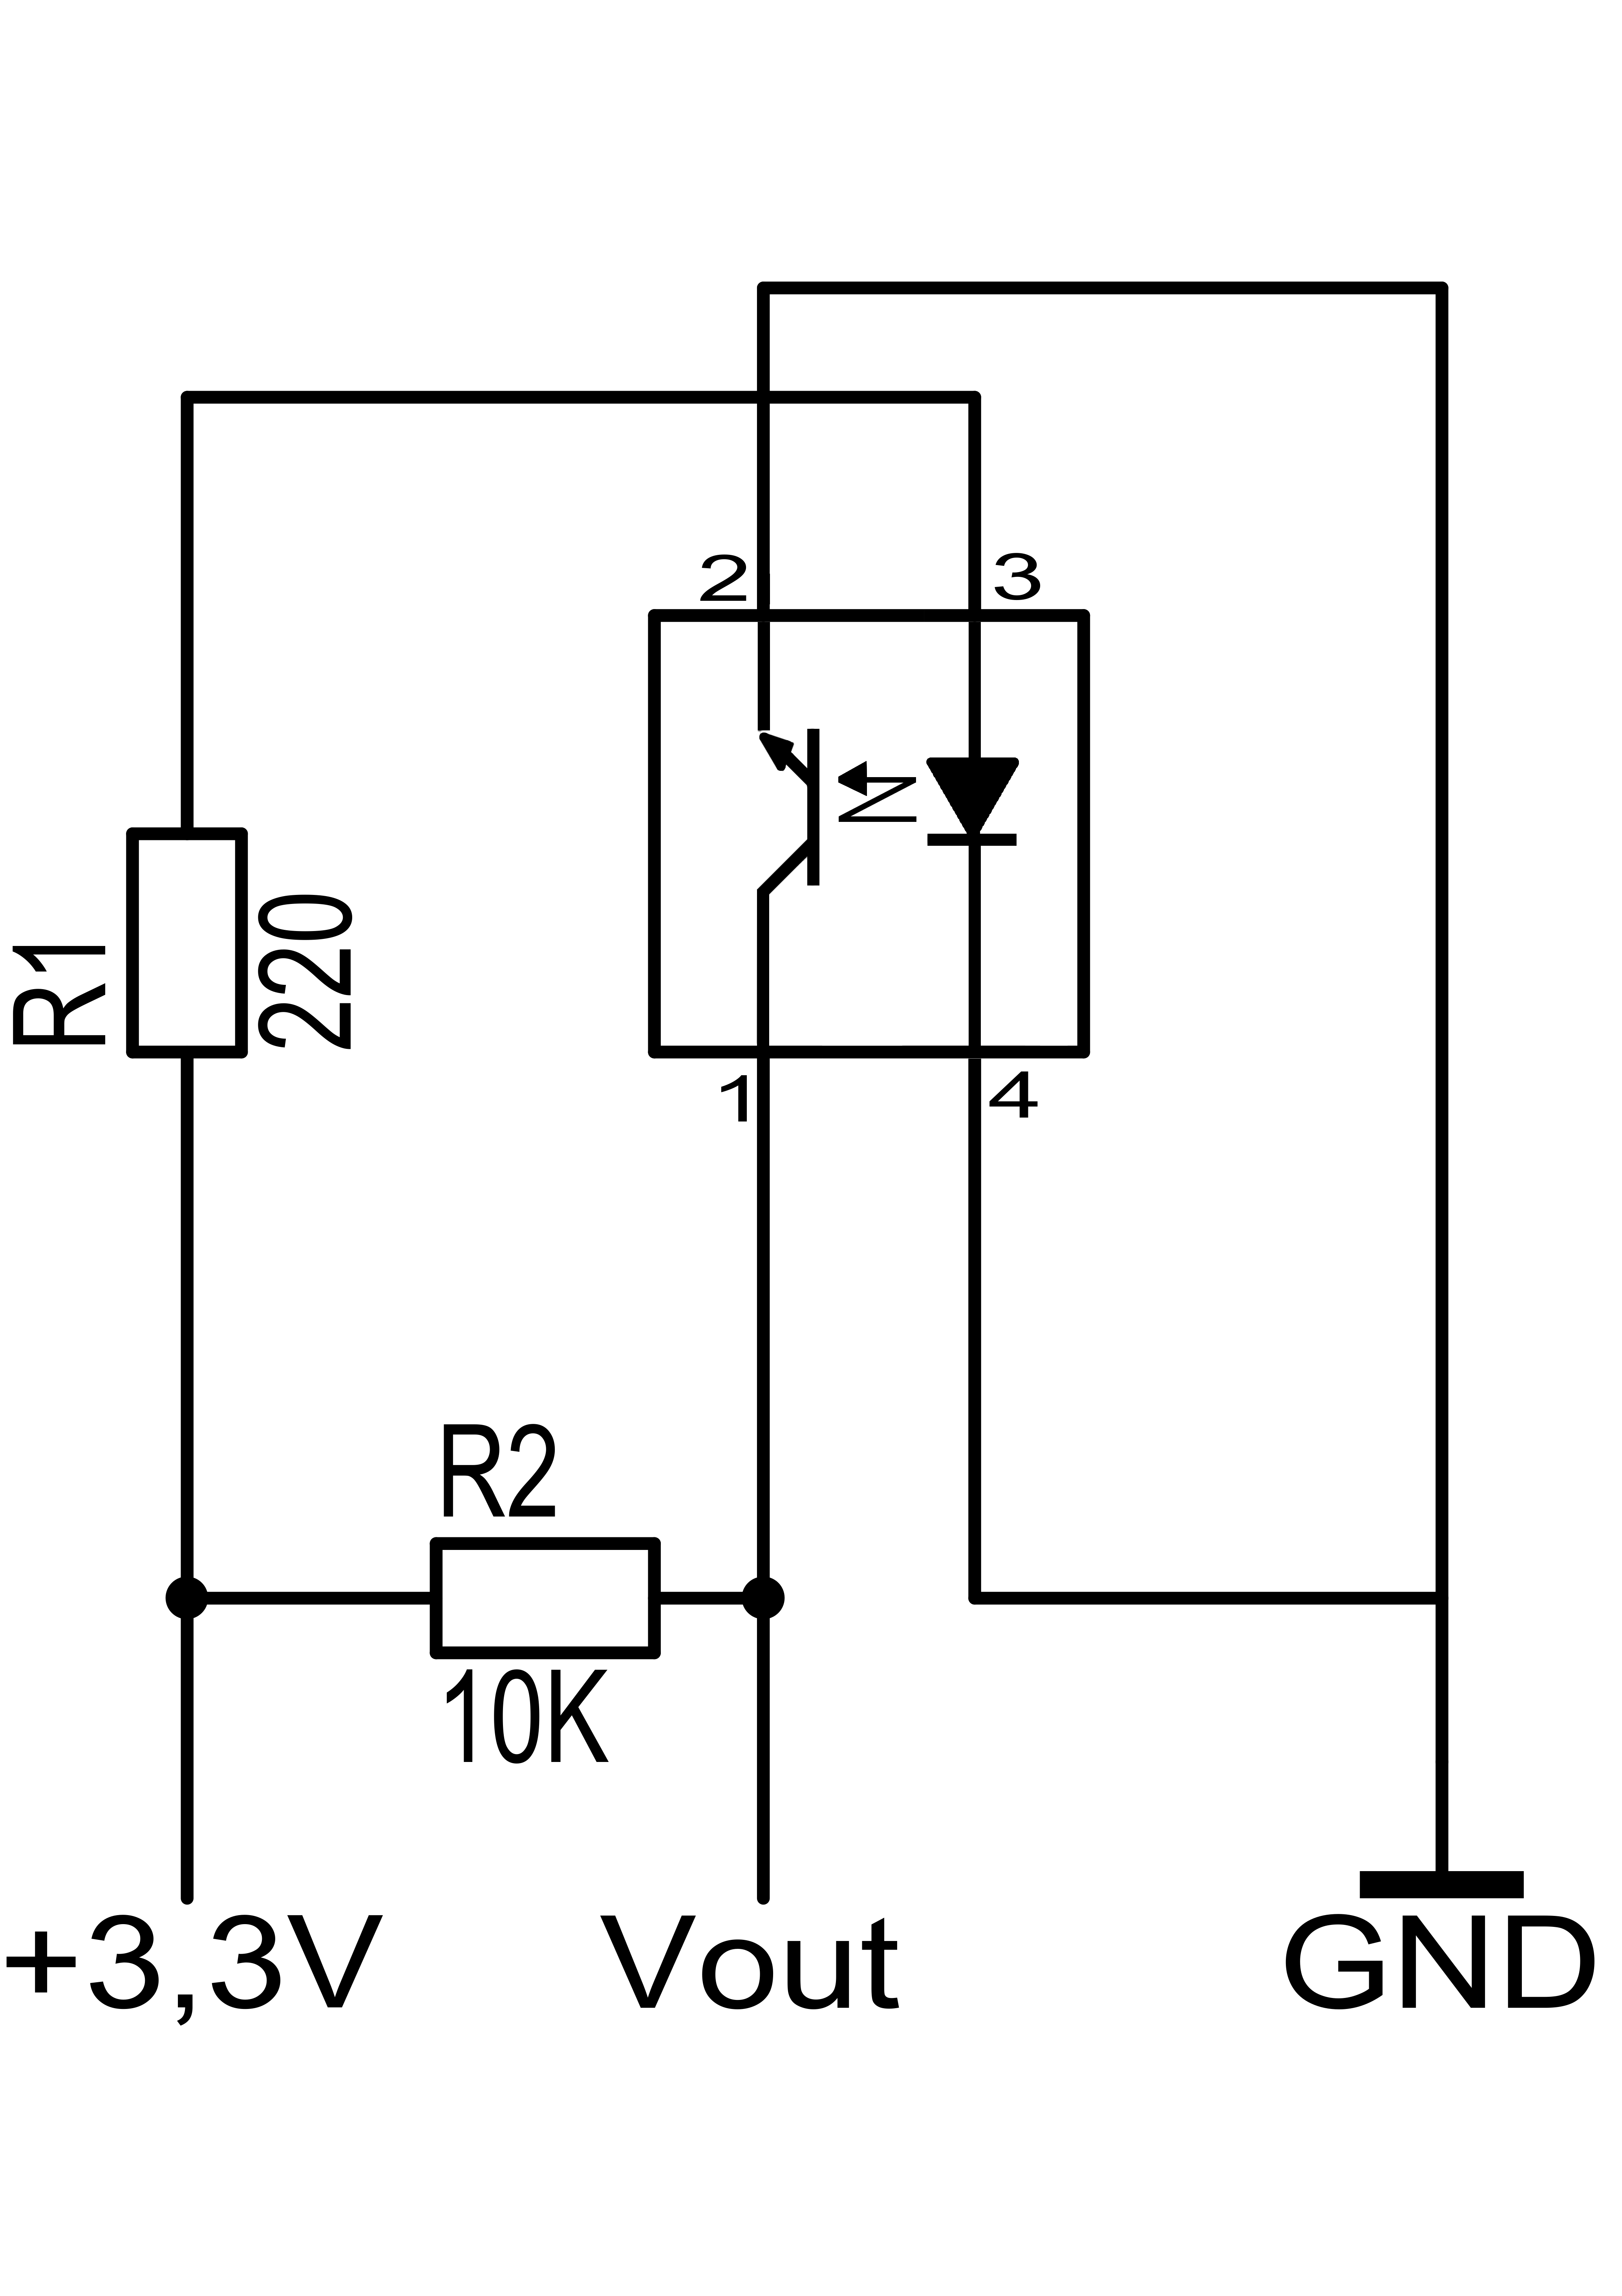
\includegraphics[scale=0.3]{immagini/QRD1114_Circuito.png}
\caption{Circuito di interfaccia tra Arduino Due e il sensore QRD1114} 
\end{figure}
\\Il circuito alimenta il LED tramite una resistenza da 220$\Omega$ (\textit{R1}) 
e collega $V_{CC}$\footnote{pari a 3,3 $V$ nell'Arduino Due.} al collettore del 
fototransistor tramite una resistenza da 10 $k\Omega$ (\textit{R2}) mentre 
l'emettitore è collegato a terra; il punto da cui prelevare il segnale ($V_{out
}$) è tra \textit{R2} e il collettore. Il principio alla base del circuito è: 
il LED è sempre acceso e illumina in modo diffuso parallelamente al 
fototransistor. Il fototransistor in assenza di luce o, nel nostro caso, in 
presenza di una bassa riflessività si trova in stato di interdizione; i pin di 
Arduino impostati come input sono in configurazione ``alta impedenza'', 
equivalenti ad un interruttore aperto dal punto di vista circuitale, quindi 
non c'è passaggio di corrente né tramite il transistor né tramite la 
resistenza \textit{R2} il che porta esattamente il valore di $V_{CC}$ in 
ingresso ad Arduino. Quando il fototransistor è totalmente illuminato, cioè in 
presenza di alta riflessività, entra in stato di conduzione così che nel punto 
$V_{out}$ si venga a trovare la massa. Ogni stato intermedio di illuminazione 
equivale ad una conduzione parziale del fototransistor a cui corrisponde una 
tensione proporzionale alla riflessività sul pin $V_{out}$. Il sensore può 
essere utilizzato in modalità digitale o analogica semplicemente collegando il 
pin $V_{out}$ ad un pin digitale o analogico e cambiando la configurazione 
relativa all'interno della programmazione di Arduino. La configurazione 
digitale si è rivelata inadatta all'applicazione in quanto risulta troppo sensibile a piccole variazioni. 
In tal caso, anche un minimo movimento sul piano verticale causato da una superficie non perfettamente piana, 
potrebbe causare un allarme di sconfinamento del robot. La configurazione 
analogica invece ci permette di avere 1024 valori discreti dal 
trasduttore, che potranno essere confrontati con un valore soglia oltre al 
quale il robot rileva un allarme di sconfinamento. La libertà nello scegliere 
una soglia di allarme ci permette di effettuare una calibrazione affinata in 
base al materiale su cui si svolge la sperimentazione per minimizzare la possibilità di 
falsi positivi. 
\subsection{Sensore di distanza a ultrasuoni - HC-SR04}
L'algoritmo di governo del robot, necessita della distanza degli oggetti che si 
trovano di fronte ad esso; la scelta è ricaduta su un sensore 
ad ultrasuoni piuttosto che su un sensore ad infrarossi in quanto quest'ultimo è
soggetto a rumore dovuto all'illuminazione dell'ambiente di sperimentazione.
In particolare abbiamo scelto il sensore HC-SR04 che 
offre ottime prestazioni, è facile da integrare ed è di dimensioni contenute.\\
Il sensore può rilevare oggetti distanti da 2 cm a 400 cm con una risoluzione 
di 0,3 cm entro un cono frontale con apertura di 60$^\circ$, 30$^\circ$ per lato 
rispetto alla perpendicolare dal sensore.
\begin{figure}[!htb] \center
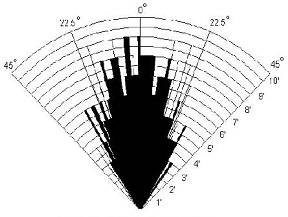
\includegraphics[scale=0.6]{immagini/HC-SR04_Angle.png}
\caption{Risposta del sensore rispetto alla posizione dell'ostacolo} 
\end{figure}
\\Il collegamento alla piattaforma di sviluppo è effettuato tramite quattro pin: 
\textit{$+5V$}, \textit{trig}, \textit{echo} e \textit{GND}.
Una volta alimentato il sensore, Arduino invia
sul pin \textit{trig} un impulso di durata $10 \mu$s; il sensore emette 
quindi un impulso ultrasonico e restituisce sul pin \textit{echo} un segnale 
positivo di durata pari al tempo di percorrenza, andata e ritorno, del segnale 
ultrasonico. Una volta ottenuto il tempo di percorrenza si utilizza la formula 
del moto rettilineo uniforme:
$$v = \frac{\Delta s}{\Delta t}$$
sapendo che la velocità del suono a 20 $^\circ$C è approssimabile a 344 m/s allora 
la durata dell'impulso di $echo$ sarà compreso tra 116.3 $\mu$s e 23,26 ms 
rispettivamente per distanze percorse di 4 cm (2+2) e di 8 m (4+4).
\\Per ricavare la distanza ($d$) in centimetri a partire dalla durata dell'impulso 
notando che 344 m/s = 29,1 cm/$\mu$s e indicando con $T_e$ la durata dell'impulso 
di echo usiamo:
$$d=\frac{T_e}{2\cdot29,1}$$
Arduino Due non accetta input a 5 V, tali valori di tensione comprometterebbero in modo 
irreparabile il funzionamento della scheda.\\ 
In questo caso il circuito di interfaccia porterà la tensione di 5 V del segnale in uscita 
dal sensore ad un valore accettato dall'Arduino Due e cioè 3,3 V; serve quindi un 
partitore di tensione.
\begin{figure}[!htb] \center
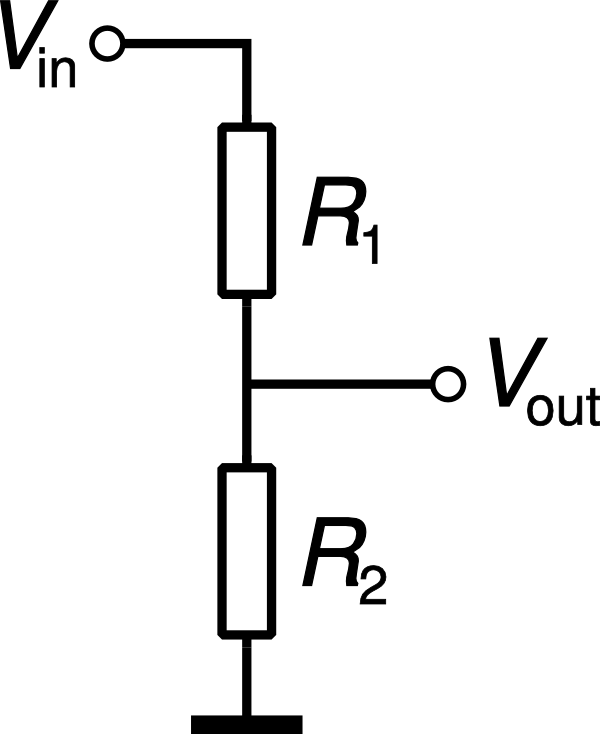
\includegraphics[scale=0.6]{immagini/Voltage_divider.png}
\caption{Schema generico del partitore di tensione} 
\end{figure}

Il partitore di tensione, a fronte di un noto valore di tensione di ingresso 
$V_{in}$, riesce a fornire il valore di tensione desiderato in uscita $V_{out}$ 
tramite due resistenze opportunamente dimensionate. \\
La formula che regola il partitore di tensione è la seguente:
$$V_{out}=V_{in}\cdot\frac{R_2}{R_1+R_2}$$
nel nostro caso $V_{in}$ = 5 V e $V_{out}$ = 3,3 V quindi scegliendo arbitrariamente 
il valore di $R_1=1$ k$\Omega$ ricaviamo il valore di $R_2$ tramite 
la formula inversa $$R_2 = R_1\cdot\frac{V_{out}}{V_{in}-V_{out}}$$
che da come risultato 1941,48 $\Omega$; approssimando il valore appena calcolato
al più vicino taglio standard di resistenze, cioè $R_2 $ = 2 k$\Omega$, si 
ottiene $V_{out}$
 = $3,\overline{3}$ che è assolutamente accettabile.

\begin{figure}[H] \center
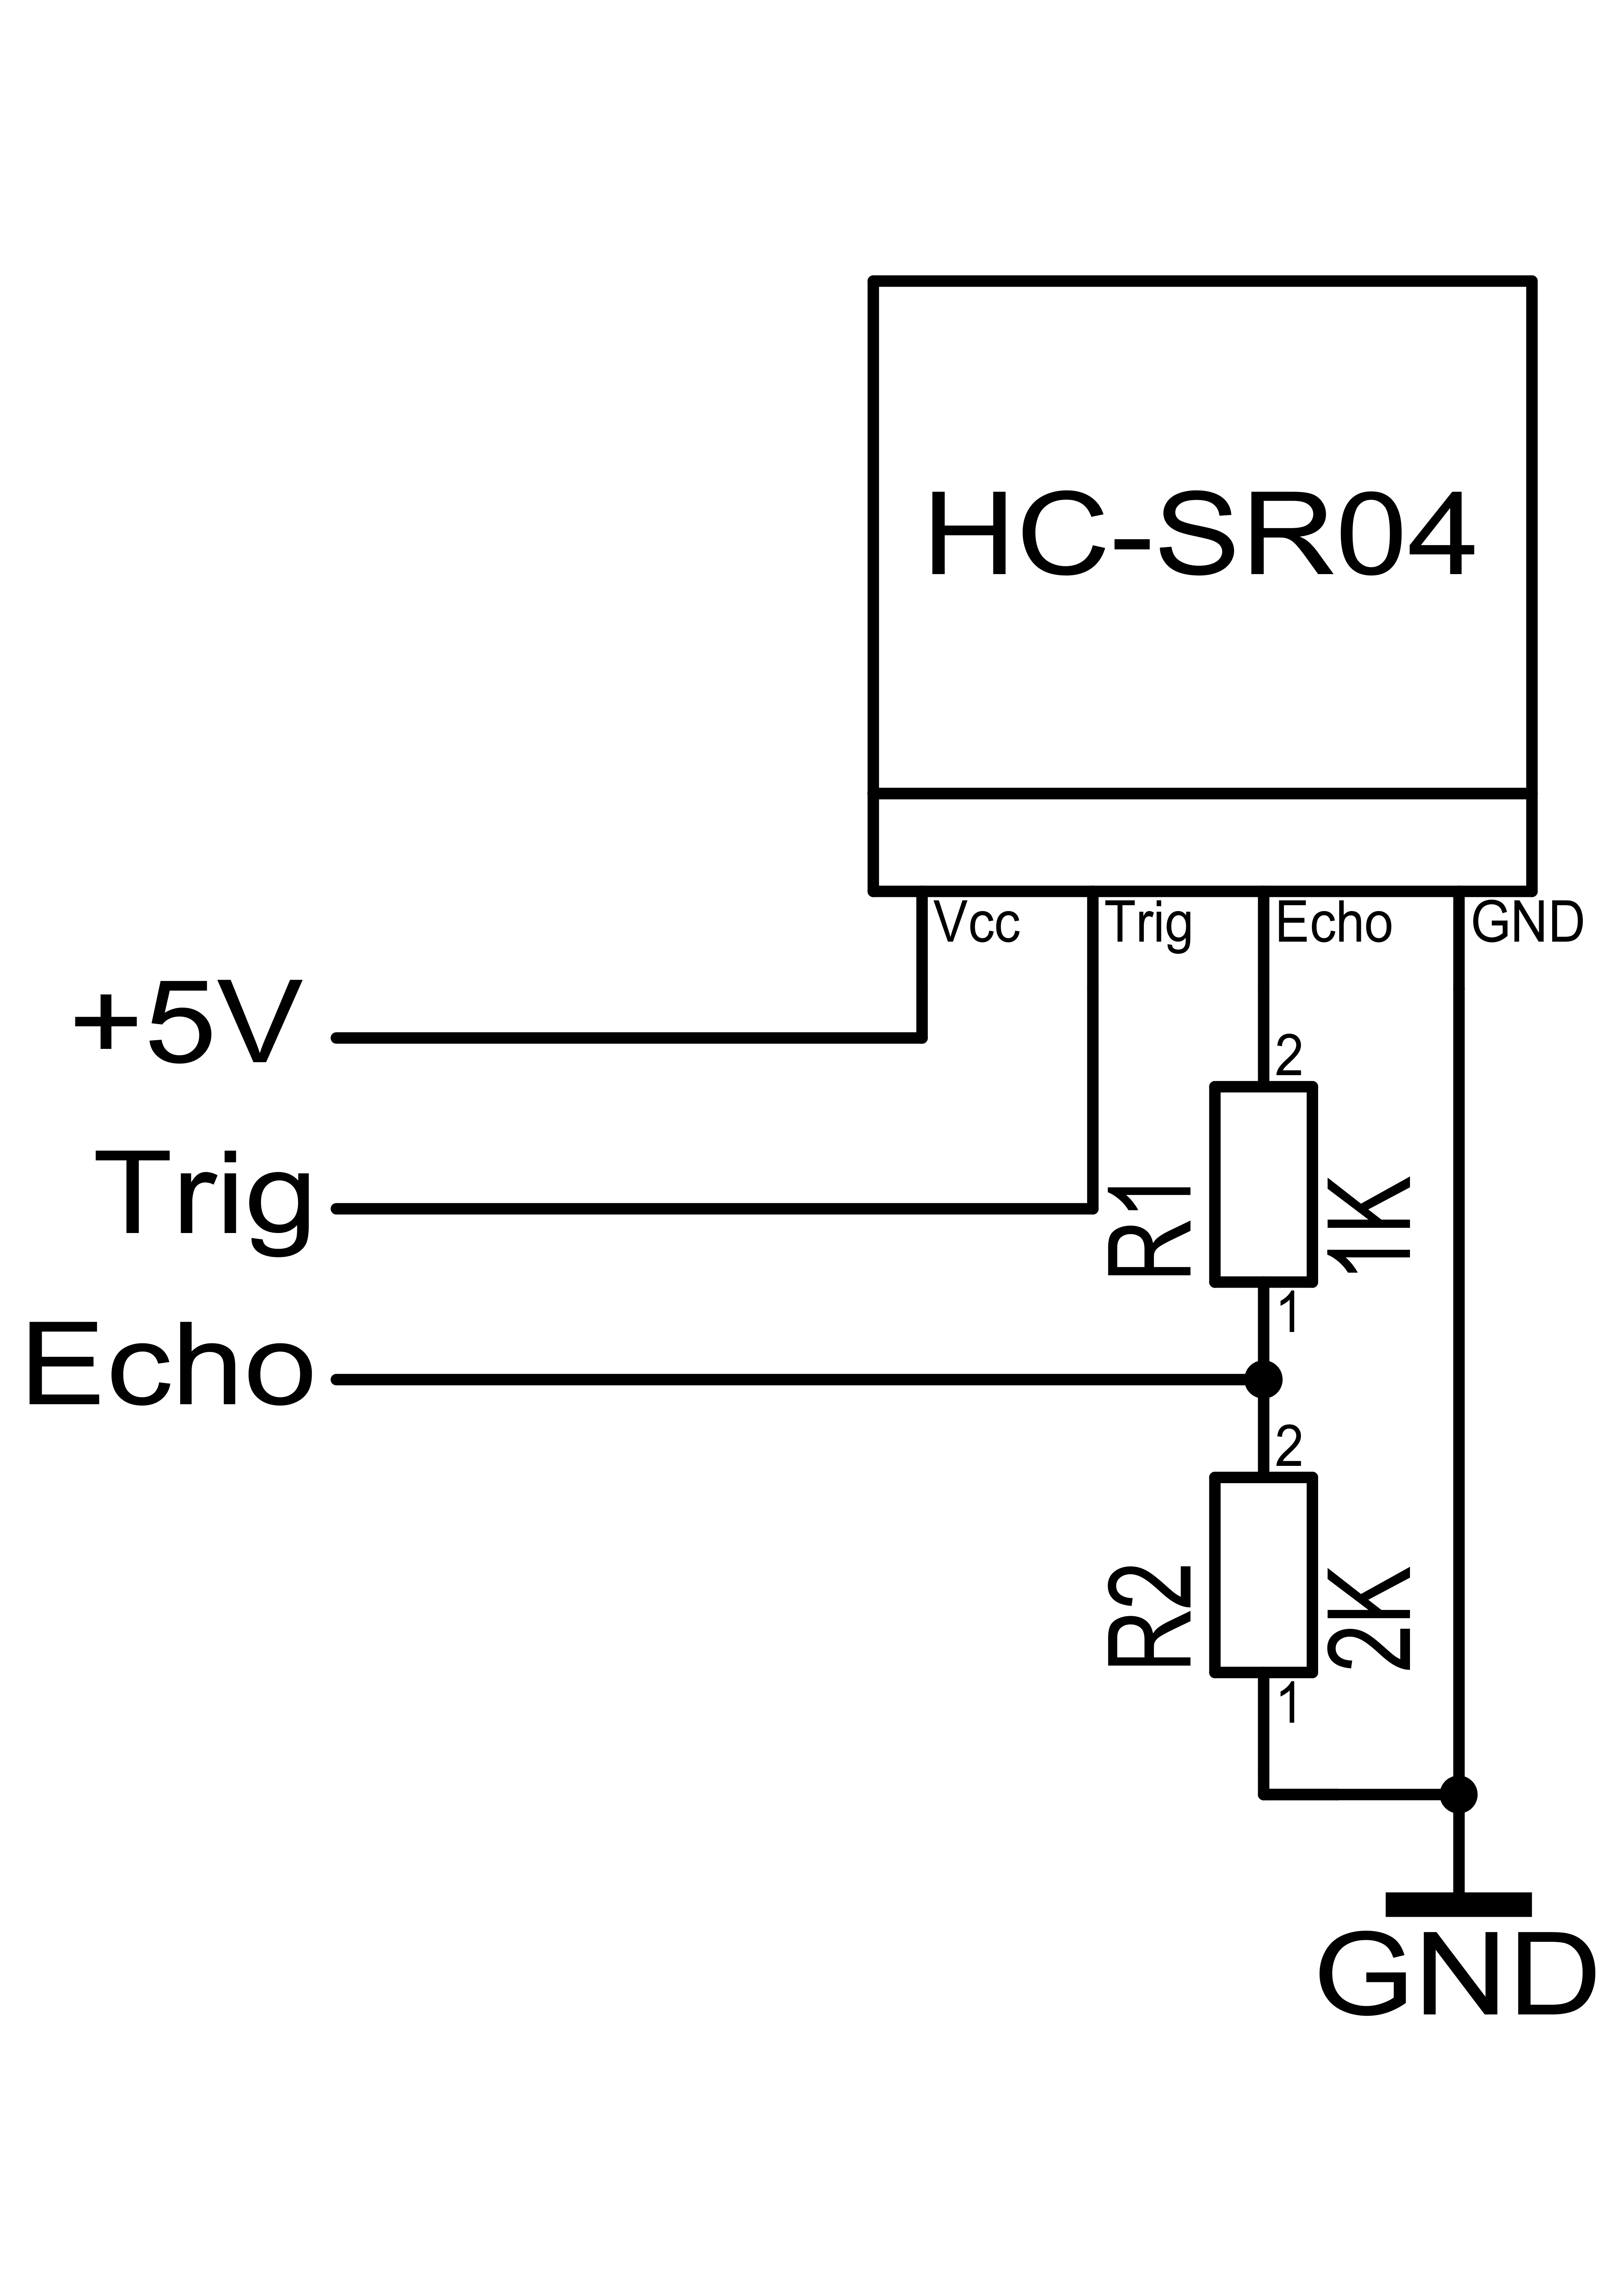
\includegraphics[scale=0.3]{immagini/HC-SR04_Circuito.png}
\caption{Circuito di interfaccia tra Arduino Due e il sensore HC-SR04} 
\end{figure}

